\section{Movimentação do manipulador robótico}
\label{sec_movimentacao_mr}

Após a estabilização da posição relativa e da atitude do perseguidor em relação ao alvo, inicia-se a etapa de movimentação do \gls{mr}  (\gls{mr}). 
Nessa fase, o objetivo é conduzir o efetuador final (\gls{eef}) até a porta de acoplamento da espaçonave alvo, permitindo a realização da atracação.

O \gls{mr} é composto por uma cadeia serial de juntas revolutas responsáveis por posicionar o \gls{eef} na porta de acoplamento. 
Essa estrutura define o espaço de trabalho do \gls{mr} e os graus de liberdade disponíveis.
Sua movimentação é calculada a partir do modelo cinemático do sistema, que relaciona as variáveis articulares do \gls{mr} com a posição e orientação do efetuador final. 
Com base nessa relação, é possível determinar as configurações articulares necessárias para conduzir o efetuador final até a porta de acoplamento.

A implementação do controle do \gls{mr} no ambiente de simulação foi realizada no Simulink, conforme ilustrado na Figura~\ref{fig_simulink_controle_mr}. 
Nesse modelo, os blocos responsáveis pela cinemática e pelo controle das juntas geram as trajetórias articulares necessárias para posicionar o efetuador final na interface de acoplamento.

\begin{figure}[H]
\centering
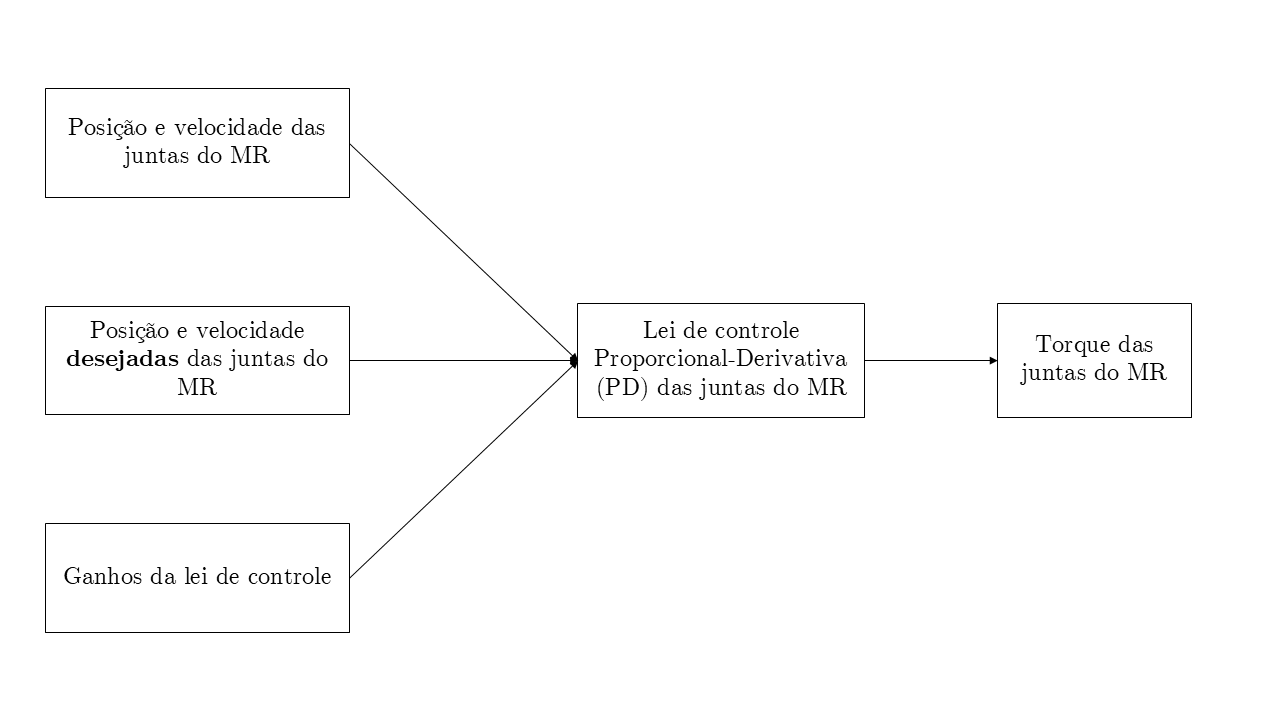
\includegraphics[width=1\linewidth]{3 Procedimento simulacao/Imagens simulink/app_final_controle_mr.png}
\caption{Modelo cinemático e do controle do \gls{mr}  no ambiente Simulink.}
\label{fig_simulink_controle_mr}
\end{figure}

Durante essa etapa, o sistema de controle de atitude da espaçonave permanece ativo, compensando os torques gerados pela movimentação das juntas do \gls{mr} e garantindo a manutenção do alinhamento entre o perseguidor e o alvo.


%%%%%%%%%%%%%%%% TORQUE REACAO ESPACONAVE

\section{Reação da espaçonave}
\label{subsec_reacao_espaconave_mr}

Durante a movimentação do \gls{mr}, os torques gerados pelas acelerações das juntas são transmitidos para a espaçonave, produzindo torques de reação que afetam diretamente sua dinâmica de atitude. 
Esse fenômeno ocorre devido ao acoplamento dinâmico entre a espaçonave e o \gls{mr}, uma vez que ambos fazem parte de um único sistema mecânico.

Para representar esse efeito na simulação, foi implementado um bloco responsável pelo cálculo do torque de reação gerado pelo movimento do \gls{mr}. 
Esse bloco utiliza como entradas as acelerações das juntas e os termos dinâmicos associados ao modelo do \gls{mr}, incluindo a matriz de inércia da espaçonave e os termos de Coriolis provenientes da formulação dinâmica baseada nas equações de Lagrange.
A Figura~\ref{fig_torque_reacao_mr} apresenta o subsistema responsável pelo cálculo do torque de reação no ambiente Simulink.

\begin{figure}[H]
\centering
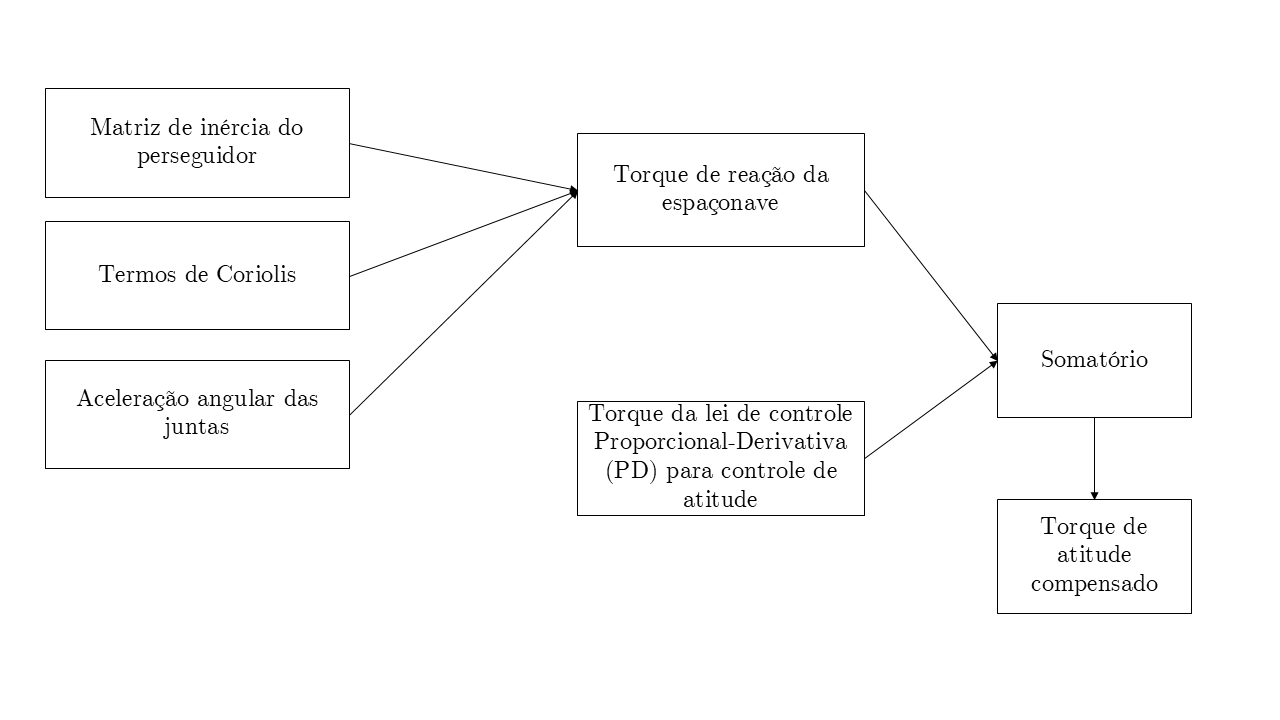
\includegraphics[width=1\linewidth]{3 Procedimento simulacao/Imagens simulink/app_final_torque_reacao.png}
\caption{Cálculo do torque de reação gerado pela movimentação do \gls{mr} .}
\label{fig_torque_reacao_mr}
\end{figure}

O torque de reação calculado é então utilizado pelo sistema de controle de atitude da espaçonave. 
Nesse processo, o torque gerado pela lei de controle \gls{pd} é combinado com o torque de reação do \gls{mr}, resultando no torque efetivamente aplicado pelos atuadores de atitude da espaçonave.

A Figura~\ref{fig_controle_pd_reacao} ilustra a implementação dessa lógica no Simulink, na qual o torque de reação é subtraído do torque calculado pelo controlador \gls{pd}, produzindo o torque compensado aplicado ao modelo dinâmico da espaçonave.

\begin{figure}[H]
\centering
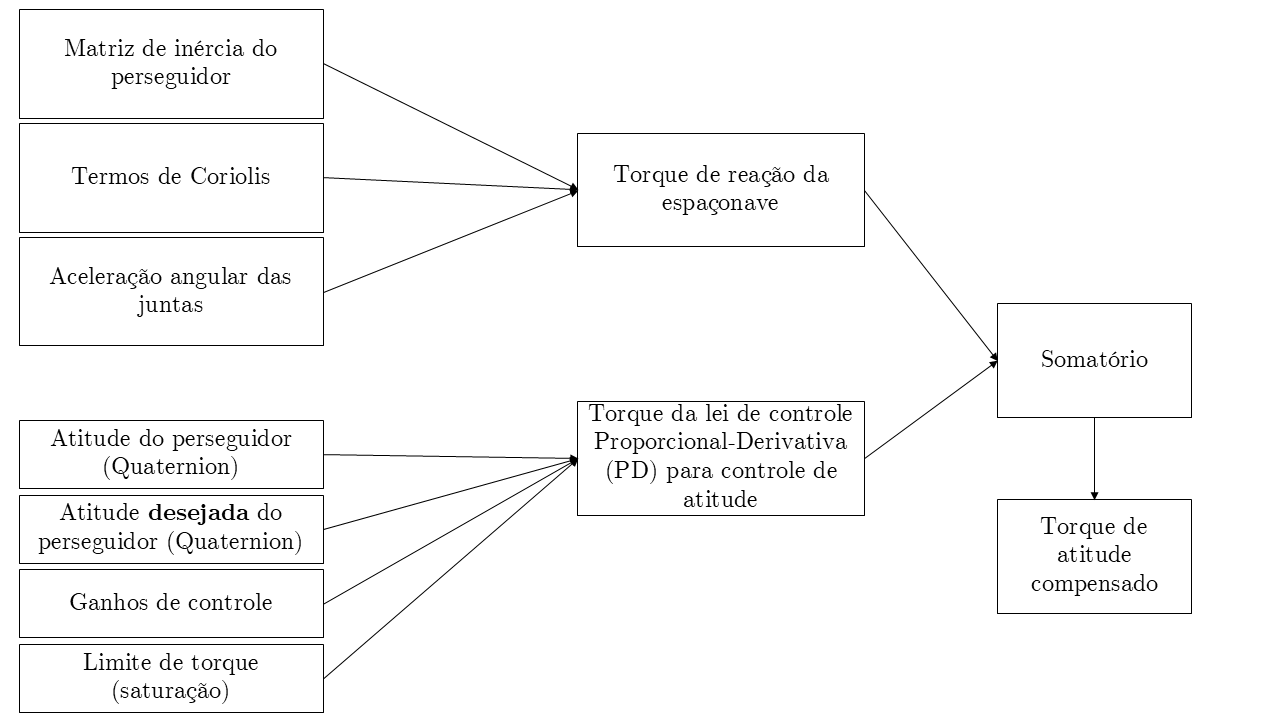
\includegraphics[width=1\linewidth]{3 Procedimento simulacao/Imagens simulink/app_final_controlePD_reacao.png}
\caption{Compensação do torque de reação do \gls{mr} no controlador de atitude da espaçonave.}
\label{fig_controle_pd_reacao}
\end{figure}

Essa estratégia permite que o sistema de controle de atitude compense automaticamente os efeitos dinâmicos introduzidos pelo movimento do \gls{mr}, contribuindo para a manutenção do alinhamento entre o perseguidor e a espaçonave alvo durante a fase de atracação.
Finalmente, é importante destacar que a relação entre as variáveis articulares do \gls{mr} e a posição do \gls{eef} é descrita pelo modelo cinemático do manipulador, apresentado no Capítulo~\ref{sec_Formulacao_Matematica}.